\section{Implementation}
Our model was implemented using PyTorch, CUDA, OptiX~\cite{parker2010optix}, and Slang~\cite{he2018slang}. 
We use OptiX to ray trace through the primitives and to provide a per-ray sorting of distances. During training we rebuild our BVH at every step, which takes tens of milliseconds.
All shaders are written in Slang~\cite{he2018slang}, a language that supports automatic differentiation with the Slang.D extension~\cite{bangaru2023slangd}. We use adjoint rendering to propagate the gradient, which means we skip storage of all function values and simply recompute them during the backwards pass.
To optimize the representation, we use our differentiable renderer in the 3DGS~\cite{kerbl20233d} codebase, and make a few adjustments to handle density based primitives (Section~\ref{sec:adc_changes} and Appendix~\ref{sec:hparams}).

\begin{figure}
    \centering
    % \includegraphics[width=0.5\textwidth]{images/blur_image.png}
    % \includegraphics[width=0.5\textwidth]{images/nottingham/00001_nottingham_fisheye.png}
    \begin{tabular}{@{}c@{}}
    \includegraphics[width=0.8\linewidth]{figures/fisheye.jpg} \\
    \small{(a) Fisheye training and rendering} \\[0.15cm]
    \includegraphics[width=0.8\linewidth]{figures/bokeh.jpg} \\
    \small{(b) Shallow depth of field rendering}
    \end{tabular}
    % \includegraphics[width=\linewidth]{figures/sidebyside.pdf}
    \vspace{-0.2cm} 
    \caption{A depiction of two benefits of ray tracing.}
    \label{fig:blur_fisheye}
\end{figure}

\subsection{Ray Tracing (BVHs) for Sorting}\label{sec:bvh}

We use ray tracing to sort primitives since it offers more flexibility than a rasterization approach like StP~\cite{radl2024stopthepop}. Ray tracing allows for effects like fisheye projection and defocus blur (see Figure~\ref{fig:blur_fisheye}) as well as random pixel offsets during training, which we find improves performance.

We start by providing the NVIDIA OptiX~\cite{parker2010optix} framework with an Axis-Aligned Bounding Box (AABB) for the ellipsoid, which is used to construct a binary tree. We then provide an intersection test to refine the search if a ray hits the bounding box, for which we adapt the stable isotropic ray/sphere intersection described by Haines et al~\cite{Haines2019}.
To further accelerate rendering, we also integrate the recent approach of 3DGRT~\cite{moenne20243d}, which accumulates multiple hits within a queue during each call to OptiX trace. 

BVH efficiency depends strongly on how often the bounding boxes of primitives overlap. Rotated anisotropic primitives tend to have large axis-aligned bounding boxes that slow down rendering. To ameliorate this, we impose a loss during training to discourage overly anisotropic primitives:
\begin{equation}
    \!\operatorname{stopgrad}\lft(1-\alpha\rgt)\lft(\max\lft(s_x, s_y, s_z\rgt) - \min\lft(s_x, s_y, s_z\rgt)\rgt),\!
\end{equation}
where $\alpha\in[0,1]$ is the opacity and  $\mathbf{s}\in \mathbb{R}^3$ is the ellipsoid axis scaling vector for each primitive.
This regularizer is applied only to primitives that are visible in the current batch. %We also bound the maximum size of primitives to 25 to further increase performance.


% We retrieve a list of sorted primitives along each ray, we collect a sorted buffer of both front and back faces using the anyhit shader. When the anyhit shader encounters a primitive that is further than the furthest primitive in the buffer, the collection terminates and the raygen shader processes the sorted buffer, before starting the next traversal, with the origin starting at the last primitive in the buffer. This algorithm~\cite{moenne20243d} is much faster than a naive algorithm that traces a ray to the closest primitive, then moves the origin before tracing another ray. However, it relies on the traversal of the anyhit shader being well behaved, and its accuracy depends on the number of overlaps and the buffer size, which we set to 16. In practice, it seems to get the same results as the naive algorithm, with a 3x speedup.

\subsection{Changes to Adaptive Density Control} \label{sec:adc_changes}

The Adaptive Density Control (ADC) used by 3DGS is critical to its success.
During training 3DGS uses a variety of strategies for periodically cloning, splitting, and pruning 3D Gaussians.
This is essential to avoid local minima by creating primitives where they are necessary and removing primitives where they are invisible.
Though these heuristics were developed specifically for 3DGS, they work well for our method with some minor necessary adjustments.

To decide where to create primitives, 3DGS accumulates the $xy$ gradients of each primitive, then splits or clones them if they are above a certain threshold every $n$ steps.
The spatial gradients of our model tend to be smaller, so the thresholds used by these splitting and cloning heuristics must be modified (splitting is $2.5\times10^{-7}$, cloning is $0.1$).
%Because reducing the threshold for cloning causes primitives to stack up on top of each other, we reduce the splitting threshold but increase the cloning one.
We use a similar splitting method as 3DGS: the primitive size is reduced and the new position is perturbed by some random amount sampled from a normal distribution, but we additionally also divide the density in half, similar to~\cite{bulo2024revising}.

% Pruning and opacity resets are designed to adaptively remove primitives from regions where they are not necessary. 
% For our method, when pruning primitives by opacity, it is important to prune by minor axis opacity because otherwise the optimization has a tendency to accumulate a large number of low opacity primitives that eat up computation. 



\section{Results}

\begin{table*}[t!]
    \centering
    \resizebox{\linewidth}{!}{
        \begin{tabular}{l|rrr|rrr|rrr}
                                     & \multicolumn{3}{c|}{Mip-NeRF360}                                                                                                      & \multicolumn{3}{c|}{Zip-NeRF}                                                                                             & \multicolumn{3}{c}{Tanks\&Temples \& DeepBlending}                                                                       \\
                                     & \multicolumn{1}{l}{PSNR $\uparrow$}                 & \multicolumn{1}{l}{SSIM $\uparrow$}   & \multicolumn{1}{l|}{LPIPS $\downarrow$} & \multicolumn{1}{l}{PSNR $\uparrow$}     & \multicolumn{1}{l}{SSIM $\uparrow$}   & \multicolumn{1}{l|}{LPIPS $\downarrow$} & \multicolumn{1}{l}{PSNR $\uparrow$}     & \multicolumn{1}{l}{SSIM $\uparrow$}   & \multicolumn{1}{l}{LPIPS $\downarrow$} \\ \hline
3DGS~\cite{kerbl20233d}              & \cellcolor[HTML]{FFFFB4}27.48                       & \cellcolor[HTML]{FFFFB4}.816          & .216                                    & 25.84                                   & .817                                  & .358                                    & \cellcolor[HTML]{FFB3B3}26.65           & \cellcolor[HTML]{FFFFB4}.848          & .263                                   \\
StopThePop~\cite{radl2024stopthepop} & 27.33                                               & \cellcolor[HTML]{FFFFB4}.816          & .212                                    & \cellcolor[HTML]{FFFFB4}25.92           & \cellcolor[HTML]{FFFFB4}.819          & \cellcolor[HTML]{FFFFB4}.352            & \cellcolor[HTML]{FFD9B3}26.60           & .847                                  & \cellcolor[HTML]{FFFFB4}.252           \\
3DGRT~\cite{moenne20243d}            & 27.20                                               & \cellcolor[HTML]{FFD9B3}.818          & \cellcolor[HTML]{FFFFB4}.248            & -                                       & -                                     & -                                       & 26.22                                   & \cellcolor[HTML]{FFD9B3}.865          & \cellcolor[HTML]{FFD9B3}.254           \\
SMERF~\cite{duckworth2024smerf}      & \cellcolor[HTML]{FFB3B3}27.99                       & \cellcolor[HTML]{FFD9B3}.818          & \cellcolor[HTML]{FFD9B3}.238            & \cellcolor[HTML]{FFB3B3}27.28           & \cellcolor[HTML]{FFD9B3}.829          & \cellcolor[HTML]{FFD9B3}.339            & -                                       & -                                     & -                                      \\
Our model                            & \cellcolor[HTML]{FFD9B3}27.51                       & \cellcolor[HTML]{FFB3B3}.825          & \cellcolor[HTML]{FFB3B3}.194            & \cellcolor[HTML]{FFD9B3}26.58           & \cellcolor[HTML]{FFB3B3}.845          & \cellcolor[HTML]{FFB3B3}.308            & \cellcolor[HTML]{FFFFB4}26.59           & \cellcolor[HTML]{FFB3B3}.889          & \cellcolor[HTML]{FFB3B3}.234           \\ \hline
ZipNeRF~\cite{barron2023zip}         & 28.54                                               & .828                                  & .198                                    & 27.37                                   & .836                                  & .305                                    & -                                       & -                                     & -                                      \\
                                     & \multicolumn{1}{l}{GPU-hr $\downarrow$}             & \multicolumn{1}{l}{Mem. $\downarrow$} & \multicolumn{1}{l|}{FPS $\uparrow$}     & \multicolumn{1}{l}{GPU-hr $\downarrow$} & \multicolumn{1}{l}{Mem. $\downarrow$} & \multicolumn{1}{l|}{FPS $\uparrow$}     & \multicolumn{1}{l}{GPU-hr $\downarrow$} & \multicolumn{1}{l}{Mem. $\downarrow$} & \multicolumn{1}{l}{FPS $\uparrow$}     \\ \hline
3DGS~\cite{kerbl20233d}              & {\color[HTML]{212121} 0.54}                         & 763MB                                 & 224                                     & 1.07                                    & 222MB                                 & 559                                     & 0.34                                    & 563MB                                 & 560                                    \\
StopThePop~\cite{radl2024stopthepop} & \cellcolor[HTML]{FFFFFF}{\color[HTML]{212121} 0.60} & 780MB                                 & 180                                     & 0.24                                    & 223MB                                 & 403                                     & 0.39                                    & 549MB                                 & 179                                    \\
3DGRT~\cite{moenne20243d}            & 0.83$\textsuperscript{\textdagger}$                 & 383MB                                 & 156$\textsuperscript{\textdagger}$      & -                                       & -                                     & -                                       & 0.83$\textsuperscript{\textdagger}$     & 388MB                                 & 190$\textsuperscript{\textdagger}$     \\
SMERF~\cite{duckworth2024smerf}      & 272                                                 & 139MB                                 & 454$\textsuperscript{\textdagger}$      & 528                                     & 4108MB                                & 408$\textsuperscript{\textdagger}$      & -                                       & -                                     & -                                      \\
Our model                            & \cellcolor[HTML]{FFFFFF}{\color[HTML]{212121} 1.04} & 1134MB                                & 36                                      & 1.26                                    & 1694MB                                & 24                                      & 0.86                                    & 1173MB                                & 44                                     \\ \hline
ZipNeRF~\cite{barron2023zip}         & \cellcolor[HTML]{FFFFFF}{\color[HTML]{212121} 32}   & 903MB                                 & ~0.5                                    & 48                                      & 903M                                  & ~0.5                                    & -                                       & -                                     & -                                     
\end{tabular}
    }
    % \resizebox{\linewidth}{!}{
    % \begin{tabular}{l|rrrrr}
                                     & \multicolumn{5}{c}{Mip-NeRF360}                                                                                                                                                                                             \\
                                     & \multicolumn{1}{l}{PSNR $\uparrow$} & \multicolumn{1}{l}{SSIM $\uparrow$} & \multicolumn{1}{l|}{LPIPS $\downarrow$}           & \multicolumn{1}{l}{GPU-hr $\downarrow$}             & \multicolumn{1}{l}{Mem. $\downarrow$} \\ \hline
3DGS~\cite{kerbl20233d}              & \cellcolor[HTML]{FFFFB4}27.48       & \cellcolor[HTML]{FFFFB4}.816        & \multicolumn{1}{r|}{.216}                         & {\color[HTML]{212121} 0.54}                         & 763MB                                 \\
StopThePop~\cite{radl2024stopthepop} & 27.33                               & \cellcolor[HTML]{FFFFB4}.816        & \multicolumn{1}{r|}{.212}                         & \cellcolor[HTML]{FFFFFF}{\color[HTML]{212121} 0.60} & 780MB                                 \\
3DGRT~\cite{moenne20243d}            & 27.20                               & \cellcolor[HTML]{FFD9B3}.818        & \multicolumn{1}{r|}{\cellcolor[HTML]{FFFFB4}.248} & $\approx$0.83                                       & 383MB                                 \\
SMERF~\cite{duckworth2024smerf}      & \cellcolor[HTML]{FFB3B3}27.99       & \cellcolor[HTML]{FFD9B3}.818        & \multicolumn{1}{r|}{\cellcolor[HTML]{FFD9B3}.238} & 272                                                 & 139MB                                 \\
Our model                            & \cellcolor[HTML]{FFD9B3}27.51       & \cellcolor[HTML]{FFB3B3}.825        & \multicolumn{1}{r|}{\cellcolor[HTML]{FFB3B3}.194} & \cellcolor[HTML]{FFFFFF}{\color[HTML]{212121} 1.04} & 1134MB                                \\ \hline
ZipNeRF~\cite{barron2023zip}         & 28.54                               & .828                                & \multicolumn{1}{r|}{.198}                         & \cellcolor[HTML]{FFFFFF}{\color[HTML]{212121} 32}   & -                                     \\ \hline
                                     & \multicolumn{5}{c}{Zip-NeRF}                                                                                                                                                                                                \\
                                     & \multicolumn{1}{l}{PSNR $\uparrow$} & \multicolumn{1}{l}{SSIM $\uparrow$} & \multicolumn{1}{l|}{LPIPS $\downarrow$}           & \multicolumn{1}{l}{GPU-hr $\downarrow$}             & \multicolumn{1}{l}{Mem. $\downarrow$} \\ \hline
3DGS~\cite{kerbl20233d}              & 25.84                               & .817                                & \multicolumn{1}{r|}{.358}                         & 1.07                                                & 222MB                                 \\
StopThePop~\cite{radl2024stopthepop} & \cellcolor[HTML]{FFFFB4}25.92       & \cellcolor[HTML]{FFFFB4}.819        & \multicolumn{1}{r|}{\cellcolor[HTML]{FFFFB4}.352} & 0.24                                                & 223MB                                 \\
3DGRT~\cite{moenne20243d}            & -                                   & -                                   & \multicolumn{1}{r|}{-}                            & -                                                   & \multicolumn{1}{l}{}                  \\
SMERF~\cite{duckworth2024smerf}      & \cellcolor[HTML]{FFB3B3}27.28       & \cellcolor[HTML]{FFD9B3}.829        & \multicolumn{1}{r|}{\cellcolor[HTML]{FFD9B3}.339} & 528                                                 & 4108MB                                \\
Our model                            & \cellcolor[HTML]{FFD9B3}26.58       & \cellcolor[HTML]{FFB3B3}.845        & \multicolumn{1}{r|}{\cellcolor[HTML]{FFB3B3}.308} & 1.26                                                & 1694MB                                \\ \hline
ZipNeRF~\cite{barron2023zip}         & 27.37                               & .836                                & \multicolumn{1}{r|}{.305}                         & 48                                                  & 662MB                                 \\ \hline
                                     & \multicolumn{5}{c}{Tanks\&Temples \& DeepBlending}                                                                                                                                                                          \\
                                     & \multicolumn{1}{l}{PSNR $\uparrow$} & \multicolumn{1}{l}{SSIM $\uparrow$} & \multicolumn{1}{l|}{LPIPS $\downarrow$}           & \multicolumn{1}{l}{GPU-hr $\downarrow$}             & \multicolumn{1}{l}{Mem. $\downarrow$} \\ \hline
3DGS~\cite{kerbl20233d}              & \cellcolor[HTML]{FFB3B3}26.65       & \cellcolor[HTML]{FFFFB4}.848        & \multicolumn{1}{r|}{.263}                         & 0.34                                                & 563MB                                 \\
StopThePop~\cite{radl2024stopthepop} & \cellcolor[HTML]{FFD9B3}26.60       & .847                                & \multicolumn{1}{r|}{\cellcolor[HTML]{FFFFB4}.252} & 0.39                                                & 549MB                                 \\
3DGRT~\cite{moenne20243d}            & 26.22                               & \cellcolor[HTML]{FFD9B3}.865        & \multicolumn{1}{r|}{\cellcolor[HTML]{FFD9B3}.254} & $\approx$0.83                                       & 388MB                                 \\
SMERF~\cite{duckworth2024smerf}      & -                                   & -                                   & \multicolumn{1}{r|}{-}                            & -                                                   & -                                     \\
Our model                            & \cellcolor[HTML]{FFFFB4}26.59       & \cellcolor[HTML]{FFB3B3}.889        & \multicolumn{1}{r|}{\cellcolor[HTML]{FFB3B3}.234} & 0.86                                                & 1173MB                                \\ \hline
ZipNeRF~\cite{barron2023zip}         & -                                   & -                                   & \multicolumn{1}{r|}{-}                            & -                                                   & \multicolumn{1}{l}{}                 
\end{tabular}
    % }
    \caption{Results on the 9 scenes from Mip-NeRF360~\cite{barron2021mip}, 4 large scenes from Zip-NeRF~\cite{barron2023zip} datasets, and 4 scenes from DeepBlending~\cite{hedman2018deep} and Tanks\&Temples~\cite{Knapitsch2017} combined.
    % ``GPU-hr'' indicates the number of GPU hours it takes to train a model.
    % Note that SMERF is a distillation of ZipNeRF that takes 33 hours to train on 16xA100 GPUs (almost a month on a single GPU, compared to our 1-2 hours).
    The increased sharpness and perceptual quality are reflected in the qualitative comparison in Fig.~\ref{fig:image_comparison}.
    ``GPU-hr'' indicates the number of GPU hours it takes to train a model. ``Mem.'' indicates the amount of memory the finished model consumes on disk. Variations in memory usage between 3DGS, StopThePop, 3DGRT, and our model are due to densification differences, as memory per primitive is the same.
    %The softness of the Gaussian primitives helps with PSNR, which is a metric that prefers blurrier images because of imprecise image alignment.
    % Zip-NeRF outperforms all other models on all metrics, but it is prohibitively slow to render for real-time applications ($\sim\!0.5$ FPS).
    FPS results are computed at test resolution, and results with a $\textsuperscript{\textdagger}$ were not recomputed and use different high end GPUs.
    }
    \label{tab:main_results}
\end{table*}

% \begin{table*}[t!]
%     \centering
%     % \resizebox{\linewidth}{!}{
%         \begin{tabular}{l|rr|rr|rr}
                                     & \multicolumn{2}{c|}{Mip-NeRF360}                                                             & \multicolumn{2}{c|}{Zip-NeRF}                                                    & \multicolumn{2}{c}{T\&T \& DB}                              \\
                                     & \multicolumn{1}{l}{GPU-hr $\downarrow$}             & \multicolumn{1}{l|}{Mem. $\downarrow$} & \multicolumn{1}{l}{GPU-hr $\downarrow$} & \multicolumn{1}{l|}{Mem. $\downarrow$} & \multicolumn{1}{l}{GPU-hr $\downarrow$} & \multicolumn{1}{l}{Mem. $\downarrow$} \\ \hline
3DGS~\cite{kerbl20233d}              & {\color[HTML]{212121} 0.54}                         & 763MB                                  & 1.07                                    & 222MB                                  & 0.34                                    & 563MB                                 \\
StopThePop~\cite{radl2024stopthepop} & \cellcolor[HTML]{FFFFFF}{\color[HTML]{212121} 0.60} & 780MB                                  & 0.24                                    & 223MB                                  & 0.39                                    & 549MB                                 \\
3DGRT~\cite{moenne20243d}            & $\approx$0.83                                       & 383MB                                  & -                                       & \multicolumn{1}{l|}{}                  & $\approx$0.83                           & 388MB                                 \\
SMERF~\cite{duckworth2024smerf}      & 272                                                 & 139MB                                  & 528                                     & 4108MB                                 & -                                       & -                                     \\
Our model                            & \cellcolor[HTML]{FFFFFF}{\color[HTML]{212121} 1.04} & 1134MB                                 & 1.26                                    & 1694MB                                 & 0.86                                    & 1173MB                                \\ \hline
ZipNeRF~\cite{barron2023zip}         & \cellcolor[HTML]{FFFFFF}{\color[HTML]{212121} 32}   & -                                      & 48                                      & 662MB                                  & -                                       & -                                    
\end{tabular}
%     % }
%     % \resizebox{\linewidth}{!}{
%     % \begin{tabular}{l|rrrrr}
                                     & \multicolumn{5}{c}{Mip-NeRF360}                                                                                                                                                                                             \\
                                     & \multicolumn{1}{l}{PSNR $\uparrow$} & \multicolumn{1}{l}{SSIM $\uparrow$} & \multicolumn{1}{l|}{LPIPS $\downarrow$}           & \multicolumn{1}{l}{GPU-hr $\downarrow$}             & \multicolumn{1}{l}{Mem. $\downarrow$} \\ \hline
3DGS~\cite{kerbl20233d}              & \cellcolor[HTML]{FFFFB4}27.48       & \cellcolor[HTML]{FFFFB4}.816        & \multicolumn{1}{r|}{.216}                         & {\color[HTML]{212121} 0.54}                         & 763MB                                 \\
StopThePop~\cite{radl2024stopthepop} & 27.33                               & \cellcolor[HTML]{FFFFB4}.816        & \multicolumn{1}{r|}{.212}                         & \cellcolor[HTML]{FFFFFF}{\color[HTML]{212121} 0.60} & 780MB                                 \\
3DGRT~\cite{moenne20243d}            & 27.20                               & \cellcolor[HTML]{FFD9B3}.818        & \multicolumn{1}{r|}{\cellcolor[HTML]{FFFFB4}.248} & $\approx$0.83                                       & 383MB                                 \\
SMERF~\cite{duckworth2024smerf}      & \cellcolor[HTML]{FFB3B3}27.99       & \cellcolor[HTML]{FFD9B3}.818        & \multicolumn{1}{r|}{\cellcolor[HTML]{FFD9B3}.238} & 272                                                 & 139MB                                 \\
Our model                            & \cellcolor[HTML]{FFD9B3}27.51       & \cellcolor[HTML]{FFB3B3}.825        & \multicolumn{1}{r|}{\cellcolor[HTML]{FFB3B3}.194} & \cellcolor[HTML]{FFFFFF}{\color[HTML]{212121} 1.04} & 1134MB                                \\ \hline
ZipNeRF~\cite{barron2023zip}         & 28.54                               & .828                                & \multicolumn{1}{r|}{.198}                         & \cellcolor[HTML]{FFFFFF}{\color[HTML]{212121} 32}   & -                                     \\ \hline
                                     & \multicolumn{5}{c}{Zip-NeRF}                                                                                                                                                                                                \\
                                     & \multicolumn{1}{l}{PSNR $\uparrow$} & \multicolumn{1}{l}{SSIM $\uparrow$} & \multicolumn{1}{l|}{LPIPS $\downarrow$}           & \multicolumn{1}{l}{GPU-hr $\downarrow$}             & \multicolumn{1}{l}{Mem. $\downarrow$} \\ \hline
3DGS~\cite{kerbl20233d}              & 25.84                               & .817                                & \multicolumn{1}{r|}{.358}                         & 1.07                                                & 222MB                                 \\
StopThePop~\cite{radl2024stopthepop} & \cellcolor[HTML]{FFFFB4}25.92       & \cellcolor[HTML]{FFFFB4}.819        & \multicolumn{1}{r|}{\cellcolor[HTML]{FFFFB4}.352} & 0.24                                                & 223MB                                 \\
3DGRT~\cite{moenne20243d}            & -                                   & -                                   & \multicolumn{1}{r|}{-}                            & -                                                   & \multicolumn{1}{l}{}                  \\
SMERF~\cite{duckworth2024smerf}      & \cellcolor[HTML]{FFB3B3}27.28       & \cellcolor[HTML]{FFD9B3}.829        & \multicolumn{1}{r|}{\cellcolor[HTML]{FFD9B3}.339} & 528                                                 & 4108MB                                \\
Our model                            & \cellcolor[HTML]{FFD9B3}26.58       & \cellcolor[HTML]{FFB3B3}.845        & \multicolumn{1}{r|}{\cellcolor[HTML]{FFB3B3}.308} & 1.26                                                & 1694MB                                \\ \hline
ZipNeRF~\cite{barron2023zip}         & 27.37                               & .836                                & \multicolumn{1}{r|}{.305}                         & 48                                                  & 662MB                                 \\ \hline
                                     & \multicolumn{5}{c}{Tanks\&Temples \& DeepBlending}                                                                                                                                                                          \\
                                     & \multicolumn{1}{l}{PSNR $\uparrow$} & \multicolumn{1}{l}{SSIM $\uparrow$} & \multicolumn{1}{l|}{LPIPS $\downarrow$}           & \multicolumn{1}{l}{GPU-hr $\downarrow$}             & \multicolumn{1}{l}{Mem. $\downarrow$} \\ \hline
3DGS~\cite{kerbl20233d}              & \cellcolor[HTML]{FFB3B3}26.65       & \cellcolor[HTML]{FFFFB4}.848        & \multicolumn{1}{r|}{.263}                         & 0.34                                                & 563MB                                 \\
StopThePop~\cite{radl2024stopthepop} & \cellcolor[HTML]{FFD9B3}26.60       & .847                                & \multicolumn{1}{r|}{\cellcolor[HTML]{FFFFB4}.252} & 0.39                                                & 549MB                                 \\
3DGRT~\cite{moenne20243d}            & 26.22                               & \cellcolor[HTML]{FFD9B3}.865        & \multicolumn{1}{r|}{\cellcolor[HTML]{FFD9B3}.254} & $\approx$0.83                                       & 388MB                                 \\
SMERF~\cite{duckworth2024smerf}      & -                                   & -                                   & \multicolumn{1}{r|}{-}                            & -                                                   & -                                     \\
Our model                            & \cellcolor[HTML]{FFFFB4}26.59       & \cellcolor[HTML]{FFB3B3}.889        & \multicolumn{1}{r|}{\cellcolor[HTML]{FFB3B3}.234} & 0.86                                                & 1173MB                                \\ \hline
ZipNeRF~\cite{barron2023zip}         & -                                   & -                                   & \multicolumn{1}{r|}{-}                            & -                                                   & \multicolumn{1}{l}{}                 
\end{tabular}
%     % }
%     \caption{Usage characeteristics on the 9 scenes from Mip-NeRF360~\cite{barron2021mip}, 4 large scenes from Zip-NeRF~\cite{barron2023zip} datasets, and 4 scenes from DeepBlending~\cite{hedman2018deep} and Tanks\&Temples~\cite{Knapitsch2017} combined.
%     ``GPU-hr'' indicates the number of GPU hours it takes to train a model. ``Mem.'' indicates the amount of memory the finished model consumes on disk. Variations in memory usage between 3DGS, StopThePop, 3DGRT, and our model are due to densification differences, as memory per primitive is the same.
%     }
%     \label{tab:usage}
% \end{table*}


We evaluate \acronym{} on the 9 scenes introduced in Mip-NeRF 360~\cite{barron2022mip}, the 4 scenes from DeepBlending~\cite{hedman2018deep} and Tanks\&Temples~\cite{Knapitsch2017}, and the 4 scenes introduced in Zip-NeRF~\cite{barron2023zip}. 
We use the same parameters across all scenes, except one: the size threshold for splitting and cloning is adjusted for large scenes to avoid total densification failure for both 3DGS and our method. For the \scenename{alameda} scene, we use the exposure trick introduced in~\cite{duckworth2024smerf} to allow evaluation on data sets with multiple exposures. We also re-tuned 3DGS to work slightly better than the tune done by Duckworth et al.~\cite{duckworth2024smerf} on the Zip-NeRF dataset.
We evaluate \acronym{} on the 9 scenes introduced in Mip-NeRF 360~\cite{barron2022mip}, the 4 scenes from DeepBlending~\cite{hedman2018deep} and Tanks\&Temples~\cite{Knapitsch2017}, and the 4 scenes introduced in Zip-NeRF~\cite{barron2023zip}. 
We use the same parameters across all scenes, except one: the size threshold for splitting and cloning is adjusted for large scenes to avoid total densification failure for both 3DGS and our method. For the \scenename{alameda} scene, we use the exposure trick introduced in~\cite{duckworth2024smerf} to allow evaluation on data sets with multiple exposures. We also re-tuned 3DGS to work slightly better than the tune done by Duckworth et al.~\cite{duckworth2024smerf} on the Zip-NeRF dataset.

% With our tuning, we are able to improve the 3DGS baseline over what was achieved by Duckworth et al.~\cite{duckworth2024smerf}, thereby providing a more fair and challenging point of comparison for our own model.

% Add scope here
There have been many follow-ups to 3DGS, each introducing different kinds of improvement, so we limit the scope of our comparison to best isolate our contribution. There are many recent approaches for densification~\cite{bulo2024revising, ververas2024sags, cao2024lightweight, ye2024absgs, yu2024gaussian}, but we chose to change densification only in ways required to handle density-based parameterization. It is likely that recent progress on improved 3DGS heuristics may similarly improve the performance of our model. There are also many different ways to change rendering~\cite{geiger2023mip, radl2024stopthepop, blanc2024, zhou2024unified, huang20242d, kheradmand20243d}, so we chose to only compare rendering methods that specifically address popping.


% , 2 scenes introduced by Tanks and Temples \cite{knapitsch2017tanks}, and 2 scenes introduced by Hedman et al. \cite{hedman2018deep}. We use the same hyperparameters for all of our experiments.



\newcommand{\graphimsix}[1]{
\begin{tikzpicture}[zoomboxarray, zoomboxarray rows=1, zoomboxes below, zoomboxarray inner gap=0.0cm]
    \node [image node] { \includegraphics[width=\figsixwidth,valign=b]{#1} };
    \zoombox[magnification=4]{0.40,0.60}
\end{tikzpicture}
}

\newcommand{\graphimseven}[1]{
\begin{tikzpicture}[zoomboxarray, zoomboxarray rows=2, zoomboxes below, zoomboxarray inner gap=0.0cm]
    \node [image node] { \includegraphics[width=\figninewidth,valign=b]{#1} };
    \zoombox[magnification=6]{0.32,0.85}
    \zoombox[magnification=10]{0.87,0.36}
\end{tikzpicture}
}

\newcommand{\graphimnine}[1]{
\begin{tikzpicture}[zoomboxarray, zoomboxarray rows=1, zoomboxes below, zoomboxarray inner gap=0.0cm]
    \node [image node] { \includegraphics[width=3.5cm,valign=b]{#1} };
    \zoombox[magnification=10]{0.5,0.5}
\end{tikzpicture}
}

\newcommand{\graphimtwo}[1]{
\begin{tikzpicture}[zoomboxarray, zoomboxarray rows=1, zoomboxes below, zoomboxarray inner gap=0.0cm]
    \node [image node] { \includegraphics[width=3.5cm,valign=b]{#1} };
    \zoombox[magnification=4]{0.45,0.30}
\end{tikzpicture}
}

\newcommand{\graphimeleven}[1]{
\begin{tikzpicture}[zoomboxarray, zoomboxarray rows=1, zoomboxes below, zoomboxarray inner gap=0.0cm]
    \node [image node] { \includegraphics[width=\figsixwidth,valign=b]{#1} };
    \zoombox[magnification=3]{0.20,0.60}
\end{tikzpicture}
}
\newcommand{\graphimtwelve}[1]{
\begin{tikzpicture}[zoomboxarray, zoomboxarray rows=1, zoomboxes below, zoomboxarray inner gap=0.0cm]
    \node [image node] { \includegraphics[width=\figsixwidth,valign=b]{#1} };
    \zoombox[magnification=4]{0.27,0.23}
\end{tikzpicture}
}
\newcommand{\graphimthirteen}[1]{
\begin{tikzpicture}[zoomboxarray, zoomboxarray rows=1, zoomboxes below, zoomboxarray inner gap=0.0cm]
    \node [image node] { \includegraphics[width=\figsixwidth,valign=b]{#1} };
    \zoombox[magnification=3]{0.45,0.45}
\end{tikzpicture}
}
\newcommand{\graphimfourteen}[1]{
\begin{tikzpicture}[zoomboxarray, zoomboxarray rows=1, zoomboxes below, zoomboxarray inner gap=0.0cm]
    \node [image node] { \includegraphics[width=\figninewidth,valign=b]{#1} };
    \zoombox[magnification=6]{0.51,0.55}
\end{tikzpicture}
}
\newcommand{\graphimfifteen}[1]{
\begin{tikzpicture}[zoomboxarray, zoomboxarray rows=1, zoomboxes below, zoomboxarray inner gap=0.0cm]
    \node [image node] { \includegraphics[width=\figsixwidth,valign=b]{#1} };
    \zoombox[magnification=4]{0.45,0.30}
\end{tikzpicture}
}

\newcommand{\graphimsixteen}[1]{
\begin{tikzpicture}[zoomboxarray, zoomboxarray rows=1, zoomboxes below, zoomboxarray inner gap=0.0cm]
    \node [image node] { \includegraphics[width=\figsixwidth cm,valign=b]{#1} };
    \zoombox[magnification=4]{0.45,0.30}
\end{tikzpicture}
}

\newcommand{\graphimseventeen}[1]{
\begin{tikzpicture}[zoomboxarray, zoomboxarray rows=1, zoomboxes below, zoomboxarray inner gap=0.0cm]
    \node [image node] { \includegraphics[width=4cm,valign=b]{#1} };
    \zoombox[magnification=4]{0.13,0.27}
\end{tikzpicture}
}


\newcommand{\graphimone}[1]{
\begin{tikzpicture}[zoomboxarray, zoomboxarray rows=1, zoomboxes below, zoomboxarray inner gap=0.0cm]
    \node [image node] { \includegraphics[width=\figninewidth,valign=b]{#1} };
    \zoombox[magnification=4]{0.225,0.55}
\end{tikzpicture}
}

\newcommand{\graphimthree}[1]{
\begin{tikzpicture}[zoomboxarray, zoomboxarray rows=1, zoomboxes below, zoomboxarray inner gap=0.0cm]
    \node [image node] { \includegraphics[width=\figninewidth,valign=b]{#1} };
    \zoombox[magnification=4]{0.15,0.25}
\end{tikzpicture}
}
\newcommand{\graphimfour}[1]{
\begin{tikzpicture}[zoomboxarray, zoomboxarray rows=1, zoomboxes below, zoomboxarray inner gap=0.0cm]
    \node [image node] { \includegraphics[width=\figninewidth,valign=b]{#1} };
    \zoombox[magnification=8]{0.85,0.83}
\end{tikzpicture}
}
\newcommand{\graphimfive}[1]{
\begin{tikzpicture}[zoomboxarray, zoomboxarray rows=2, zoomboxes below, zoomboxarray inner gap=0.0cm]
    \node [image node] { \includegraphics[width=\figninewidth,valign=b]{#1} };
    \zoombox[magnification=4]{0.35,0.90}
    \zoombox[magnification=4]{0.75,0.87}
\end{tikzpicture}
}

\newcommand{\graphimeight}[1]{
\begin{tikzpicture}[zoomboxarray, zoomboxarray rows=1, zoomboxes below, zoomboxarray inner gap=0.0cm]
    \node [image node] { \includegraphics[width=\figninewidth,valign=b]{#1} };
    \zoombox[magnification=8]{0.13,0.37}
\end{tikzpicture}
}

\begin{figure*}[ht]
\centering
\bgroup
% \resizebox{!}{\paperheight}{
% \def\arraystretch{2}
\begin{tabular}{c@{}c@{}c@{}c@{}c}
% \graphimeleven{images/comparison_table_jpg/3DGS_im11.jpg} &
% \graphimeleven{images/comparison_table_jpg/mcmc_im11.jpg} &
% \graphimeleven{images/comparison_table_jpg/stop_im11.jpg} &
% \graphimeleven{images/comparison_table_jpg/ours_im11.jpg} &
% \graphimeleven{images/comparison_table_jpg/gt_im11.jpg} \\
% \raisebox{3.0cm}{\textbf{(a)}} &
% \graphimfifteen{images/comparison_table_jpg/3DGS_im15.jpg} &
% \graphimfifteen{images/comparison_table_jpg/mcmc_im15.jpg} &
% \graphimfifteen{images/comparison_table_jpg/stop_im15.jpg} &
% \graphimfifteen{images/comparison_table_jpg/ours_im15.jpg} &
% \graphimfifteen{images/comparison_table_jpg/gt_im15.jpg} \\
% \raisebox{3.0cm}{\textbf{(c)}} &
\graphimfour{images/comparison_table_jpg/3DGS_im4.jpg} &
% \graphimfour{images/comparison_table_jpg/mcmc_im4.jpg} &
\graphimfour{images/comparison_table_jpg/stop_im4.jpg} &
% \graphimfour{images/comparison_table_jpg/3dgrt_im4.jpg} &
\graphimfour{images/comparison_table_jpg/smerf_im4.jpg} &
\graphimfour{images/comparison_table_jpg/ours_im4.jpg} &
\graphimfour{images/comparison_table_jpg/gt_im4.jpg} \\
\graphimeight{images/comparison_table_jpg/3DGS_im8.jpg} &
% \graphimeight{images/comparison_table_jpg/mcmc_im8.jpg} &
\graphimeight{images/comparison_table_jpg/stop_im8.jpg} &
% \graphimeight{images/comparison_table_jpg/3dgrt_im8.jpg} &
\graphimeight{images/comparison_table_jpg/smerf_im8.jpg} &
\graphimeight{images/comparison_table_jpg/ours_im8.jpg} &
\graphimeight{images/comparison_table_jpg/gt_im8.jpg} \\
\graphimsix{images/comparison_table_jpg/3DGS_im6.jpg} &
% \graphimsix{images/comparison_table_jpg/mcmc_im6.jpg} &
\graphimsix{images/comparison_table_jpg/stop_im6.jpg} &
% \graphimsix{images/comparison_table_jpg/3dgrt_im6.jpg} &
\graphimsix{images/comparison_table_jpg/smerf_im6.jpg} &
\graphimsix{images/comparison_table_jpg/ours_im6.jpg} &
\graphimsix{images/comparison_table_jpg/gt_im6.jpg} \\
% \raisebox{3.0cm}{\textbf{(d)}} &
% \graphimsixteen{images/comparison_table_jpg/3DGS_im16.jpg} &
% \graphimsixteen{images/comparison_table_jpg/mcmc_im16.jpg} &
% \graphimsixteen{images/comparison_table_jpg/stop_im16.jpg} &
% \graphimsixteen{images/comparison_table_jpg/ours_im16.jpg} &
% \graphimsixteen{images/comparison_table_jpg/gt_im16.jpg} \\
% \graphimseventeen{images/comparison_table_jpg/3DGS_im17.jpg} &
% \graphimseventeen{images/comparison_table_jpg/mcmc_im17.jpg} &
% \graphimseventeen{images/comparison_table_jpg/stop_im17.jpg} &
% \graphimseventeen{images/comparison_table_jpg/ours_im17.jpg} &
% \graphimseventeen{images/comparison_table_jpg/gt_im17.jpg} \\
\graphimeleven{images/comparison_table_jpg/3DGS_im11.jpg} &
% \graphimeleven{images/comparison_table_jpg/mcmc_im11.jpg} &
\graphimeleven{images/comparison_table_jpg/stop_im11.jpg} &
% \graphimeleven{images/comparison_table_jpg/3dgrt_im11.jpg} &
\graphimeleven{images/comparison_table_jpg/smerf_im11.jpg} &
\graphimeleven{images/comparison_table_jpg/ours_im11.jpg} &
\graphimeleven{images/comparison_table_jpg/gt_im11.jpg} \\
3DGS & StopThePop & SMERF & Ours & GT
\end{tabular}
% }
\egroup
\caption{Visual comparison of our method on the Mip-NeRF~\cite{barron2021mip} and Zip-NeRF~\cite{barron2023zip} datasets. Rows 1 and 2 show regions where our results are sharper. Rows 3 and 4 show how proper blending of primitives helps with handling lighting on textureless surfaces. 3DGRT is omitted due to missing Zip-NeRF results.}
\label{fig:image_comparison}
\end{figure*}


\subsection{Reconstruction Quality}
We measure image quality through the standard image metrics PSNR, SSIM and LPIPS.
% Note, however that we recompute LPIPS for all methods to ensure they use the same back-end (VGG) and input color range ($[-1,1]$).
We compare our method with 3DGS~\cite{kerbl20233d}, and with Zip-NeRF~\cite{barron2023zip}, the current offline rendering state-of-the-art for these datasets. We also compare with StopThePop since it improves view-consistency for 3DGS, 3DGRT~\cite{moenne20243d} because our work uses their ray tracing algorithm, and with SMERF~\cite{duckworth2024smerf}, because even though it is a distillation based method that takes 33 hours to train on 16xA100 GPUs compared to 1-2 hours for our method, it is a comparable real-time 3D consistent volume rendering method.

Quantitatively, we outperform the other 3DGS-based methods across the board, and set a new state of the art in the Zip-NeRF dataset in terms of sharpness as measured by LPIPS and SSIM --- even when compared to offline and distillation-based methods. 
Qualitatively, we notice two main factors: improved blending, and improved sharpness.
The combination of more flexible primitive appearance, combined with color blending, allows our method to represent gradients better, which can be seen in Figure~\ref{fig:alpha_profiles}.
This effect can also be seen when comparing how these methods model light falling on flat walls, as shown by the bottom two rows of Figure~\ref{fig:image_comparison}. 
While our method is able to reproduce the smooth image gradients in the shadowed areas, all of the Gaussian based methods struggle.
The improved sharpness is more apparent on the larger and more difficult Zip-NeRF dataset, both in the metrics and in qualitative examples (see the second two rows of Figure~\ref{fig:image_comparison}). 
%This improved sharpness is not matched by 3DGS, even when improved densification from 3DGS-MCMC is factored in.


\begin{figure*}[ht]
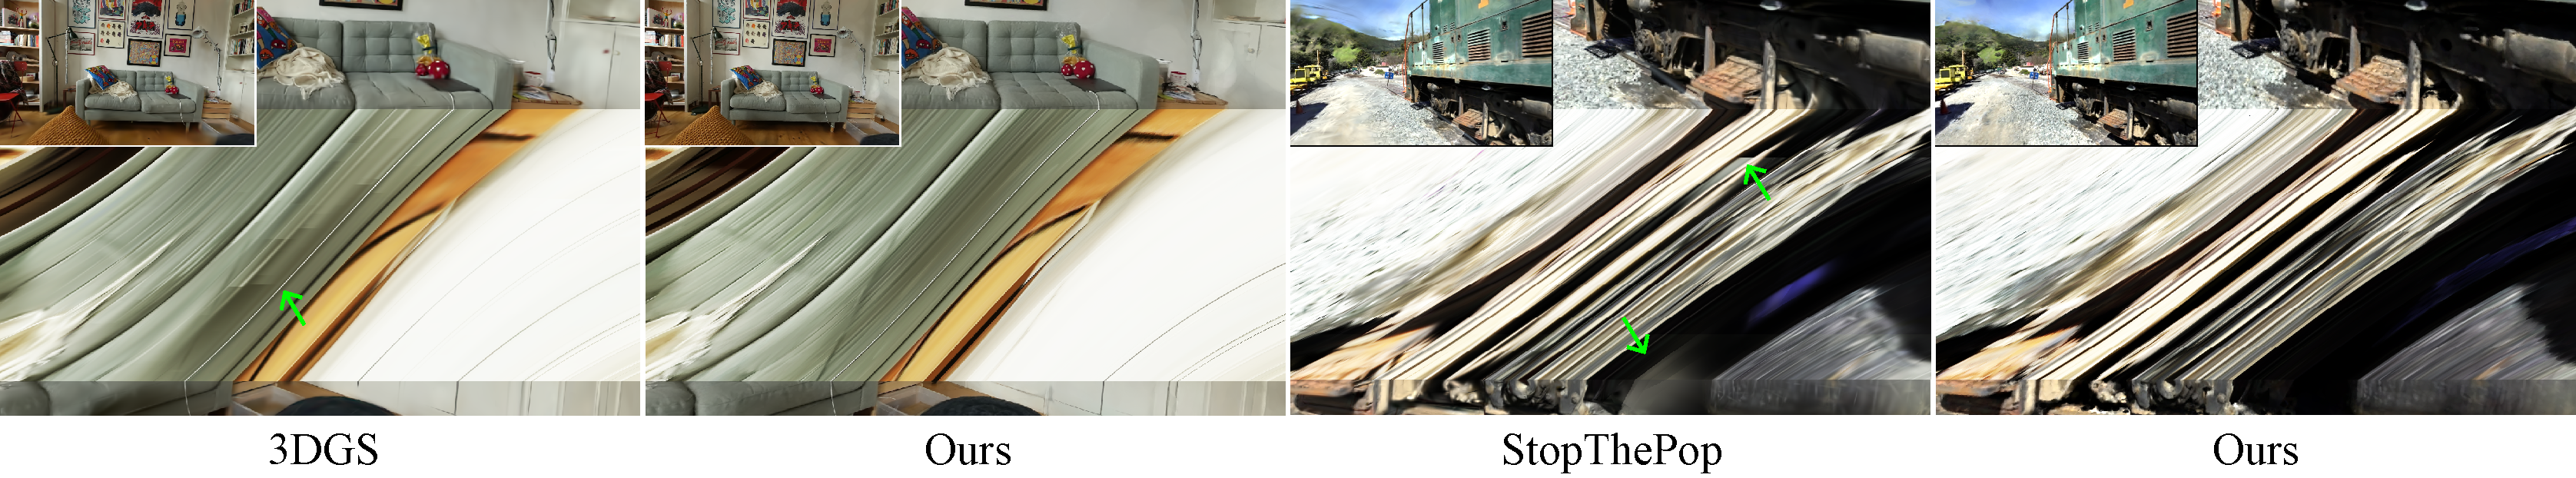
\includegraphics[width=\linewidth]{figures/EPIs_large_contrast.pdf}
\caption{
Here we show epipolar plane images \cite{bolles1987epipolar} to visualize popping in 3DGS~\cite{kerbl20233d} and StopThePop~\cite{radl2024stopthepop}. We recorded sequences of images while rotating the camera in the \scenename{berlin}~\cite{barron2023zip} (left) and \scenename{train}~\cite{knapitsch2017tanks} (right) scenes. The region in the middle are the epipolar plane images, with green arrows highlighting discontinuities in the color caused by popping/blend order artifacts. Our method lacks these horizontal discontinuities. Contrast and brightness have been boosted here for visibility's sake. See the supplemental video for more.}
\label{fig:popping_train}
\end{figure*}

\newcommand{\graphablation}[1]{
\begin{tikzpicture}[zoomboxarray]
    \node [image node] { \includegraphics[width=4.15cm]{#1} };
    \zoombox[magnification=6]{0.85,0.93}
    \zoombox[magnification=4]{0.6,0.55}
\end{tikzpicture}
}
% \begin{figure*}
%     \centering
%     \begin{tabular}{@{}cc@{}}
%     % \vspace{-3pt}
%     \graphablation{images/ablation/splatted.png} &
%     \graphablation{images/ablation/nomixing.png} \\
%     % \vspace{-3pt}
%     \small{(a) Splatted} & \small{(b) No Mixing} \\
%     \graphablation{images/ablation/ours.png} &
%     \graphablation{images/ablation/gt.png} \\
%     \small{(c) Volume Rendering (Ours)} & \small{(d) Ground Truth}
%     \end{tabular}
%     \vspace{-8pt}
%     \caption{To visualize the difference between rendering methods, we optimize our ellipsoids for our method, then visualize how different rendering methods affect the final image. Both ``Splatted'' and ``No Mixing'' assume that Gaussians do not overlap, with the former ordering them globally for the image (like 3DGS) , and the latter sorting them independently per pixel (like StopThePop). Both approaches cause hard edges to appear in areas where different primitives were blended to produce a color gradient.}
%     \label{fig:ablation}
% \end{figure*}


\subsection{Popping}

\begin{table}[b!]
\resizebox{\linewidth}{!}{
\large
\begin{tabular}{l|rr|rr|rr|rr}
StP Popping & \multicolumn{2}{l|}{DeepBlending}                                                      & \multicolumn{2}{l|}{M360 Indoor}                                                       & \multicolumn{2}{l|}{M360 Outdoor}                                                      & \multicolumn{2}{l}{Tanks \& Temples}                                                  \\
Metric      & \multicolumn{1}{l}{\reflectbox{F}LIP$_1$} & \multicolumn{1}{l|}{\reflectbox{F}LIP$_7$} & \multicolumn{1}{l}{\reflectbox{F}LIP$_1$} & \multicolumn{1}{l|}{\reflectbox{F}LIP$_7$} & \multicolumn{1}{l}{\reflectbox{F}LIP$_1$} & \multicolumn{1}{l|}{\reflectbox{F}LIP$_7$} & \multicolumn{1}{l}{\reflectbox{F}LIP$_1$} & \multicolumn{1}{l}{\reflectbox{F}LIP$_7$} \\ \hline
3DGS        & \cellcolor[HTML]{FFFFB4}0.0063            & \cellcolor[HTML]{FFFFB4}0.0122             & \cellcolor[HTML]{FFFFB4}0.0072            & \cellcolor[HTML]{FFFFB4}0.0149             & \cellcolor[HTML]{FFFFB4}0.0083            & \cellcolor[HTML]{FFFFB4}0.0154             & \cellcolor[HTML]{FFFFB4}0.0107            & \cellcolor[HTML]{FFFFB4}0.0315            \\
StopThePop  & \cellcolor[HTML]{FFD9B3}0.0052            & \cellcolor[HTML]{FFD9B3}0.0055             & \cellcolor[HTML]{FFD9B3}0.0060            & \cellcolor[HTML]{FFD9B3}0.0073             & \cellcolor[HTML]{FFD9B3}0.0083            & \cellcolor[HTML]{FFD9B3}0.0115             & \cellcolor[HTML]{FFD9B3}0.0076            & \cellcolor[HTML]{FFD9B3}0.0114            \\
Ours        & \cellcolor[HTML]{FFB3B3}0.0031            & \cellcolor[HTML]{FFB3B3}0.0000             & \cellcolor[HTML]{FFB3B3}0.0049            & \cellcolor[HTML]{FFB3B3}0.0000             & \cellcolor[HTML]{FFB3B3}0.0067            & \cellcolor[HTML]{FFB3B3}0.0000             & \cellcolor[HTML]{FFB3B3}0.0040            & \cellcolor[HTML]{FFB3B3}0.0000           
\end{tabular}
}\\
\caption{Experimental evidence that our method does not suffer popping, using the metric from StopThePop~\cite{radl2024stopthepop}. \reflectbox{F}LIP$_7$ is considered a more reliable step size by the authors because the signal is stronger than the noise caused by the optical flow used to compute the metric.}
\label{tab:popping}
\end{table}

As established in Figure~\ref{fig:popping_diagram}, both 3DGS and StopThePop exhibit artifacts due to their view-dependent density. We show what these artifacts look like using epipolar plane images \cite{bolles1987epipolar} in Figure~\ref{fig:popping_train}.
Because our rendering model is exact, and because the volume rendering integral is a continuous function of ray direction, our renderings exhibit no popping. Please see the supplemental video for a clear visualization.

To accompany our theoretical explanation of why our method does not suffer popping, we compare our method to StopThePop and 3DGS using the metric from StopThePop~(StP) to measure the amount of popping, closely following the original author's methodology across all the original scenes measured. EVER achieves a lower (better) score at step=1, and 0.0 error (lowest) with step=7, which StP called a more reliable step size, see Table.~\ref{tab:popping}. 

\subsection{Performance}
At 720p, we achieve average framerates of 36 FPS on the mip-NeRF 360 outdoor scenes, 66 FPS on the mip-NeRF 360 indoor scenes, and 30 FPS on the Zip-NeRF scenes on an NVIDIA RTX4090. The test set resolution is high on a couple of the Zip-NeRF and Mip-NeRF360 scenes, which causes the drop in FPS in Table~\ref{tab:main_results}. Training takes around 1-2 hours, also on an NVIDIA RTX4090. 
The majority of the time is spent tracing through the scene for rendering, which takes 20-71 ms, depending on the BVH.
For back propagation, 16 ms are spent storing intersections, and 13-20 ms are spent loading the primitives and atomically adding up the gradients. The BVH is rebuilt every training iteration, which takes 2-20 ms.

\newcommand{\graphimten}[1]{
\begin{tikzpicture}[zoomboxarray, zoomboxarray rows=1, zoomboxes below, zoomboxarray inner gap=0.0cm]
    \node [image node] { \includegraphics[width=4.5cm,valign=b]{#1} };
    \zoombox[magnification=4]{0.125,0.54}
\end{tikzpicture}
}

\begin{table}[b!]
\resizebox{\linewidth}{!}{
\large
\begin{tabular}{l|ccc|c}
                   & \multicolumn{1}{c}{PSNR$\uparrow$} & \multicolumn{1}{c}{SSIM$\uparrow$} & \multicolumn{1}{c|}{LPIPS$\downarrow$} & \multicolumn{1}{c}{FPS$\uparrow$}               \\ \hline
Splatted           & 26.63                               & .845                                & .329                                    & -                                                \\
No Mixing          & 26.79                               & .849                                & .305                                    & -                                                \\
3DGS               & 27.02                               & .853                                & .301                                    & -                                                \\
3DGS + Our Changes & 26.94                               & .832                                & .323                                    & -                                                \\
No Anisotropic     & \cellcolor[HTML]{FFB3B3}27.25       & \cellcolor[HTML]{FFB3B3}.865        & \cellcolor[HTML]{FFB3B3}.272            & \multicolumn{1}{r}{27.3}                         \\
No Points          & \cellcolor[HTML]{FFD9B3}27.19       & \cellcolor[HTML]{FFD9B3}.863        & \cellcolor[HTML]{FFD9B3}.277            & \multicolumn{1}{r}{\cellcolor[HTML]{FFFFB4}41.2} \\
No Rand Center     & 27.08                               & .859                                & \cellcolor[HTML]{FFFFB4}.278            & \multicolumn{1}{r}{\cellcolor[HTML]{FFD9B3}41.4} \\ \hline
Ours               & \cellcolor[HTML]{FFFFB4}27.17       & \cellcolor[HTML]{FFFFB4}.862        & \cellcolor[HTML]{FFD9B3}.277            & \multicolumn{1}{r}{\cellcolor[HTML]{FFB3B3}41.9}
\end{tabular}
}\\
\caption{
An ablation study reporting average performance on the \scenename{bicycle} and \scenename{counter} scenes from MipNeRF 360~\cite{barron2021mip} and the \scenename{berlin} scene from ZipNeRF~\cite{barron2023zip}. The ``No Anisotropic'' ablation shows the cost of our regularizer that increases frame-rate.}
\label{tab:ablation}
\end{table}

\subsection{Ablations}
To see if it was possible to train our model using ray tracing, then render using splatting, we implemented a splatting version of our 3D ellipsoids, labeled ``Splatted''. We also tested what would happen if we sorted the primitives per ray like StopThePop without our color blending technique, which is labeled ``No Mixing''. Both of these resulted in visual degradation in areas where the method had been mixing primitive colors together, which can be seen on the fridge and candle. 
These ablations also perform worse when trained for their specific rendering styles, as can be seen in Table~\ref{tab:ablation}. ``Splatting'' performs worse than ``No Mixing'', which does not match the comparison between 3DGS and StopThePop, both of which have similar performance. %This could be an indication that per ray sorting provides some kind of improved blending.

To ablate the effect of our densification changes, along with the other changes, we use the 3DGS renderer with the other minor changes we've made to densification, which we label ``3DGS + Our Changes''.
These changes do not help 3DGS because they are aimed at handling density primitives. 
Finally, we run ablations on each of the changes we performed.
``No anisotropic'' refers to ablating anisotropic loss, which results in slightly increased quality, but much lower framerate. ``No points'' refers to no additional points added using the inverse contraction, which reduces the reliance on the SfM reconstruction. The inverse contraction sampling is described in the supplemental material.
%, which has almost no effect on the quality, but is useful on datasets where the SfM wasn't very good, like London.
``No Rand Centers'' refers to ablating randomizing the pixel centers, which helps with thin structures on the bicycle scene.
We jitter our rays by picking a point within the pixel from a uniform random distribution, as opposed to using the center of the pixel. 

\section{Conclusion}

% Order of claims: 
% 1. We introduce exact volume rendering for infinite overlapping primitives in real time
% 2. We observe that this improves smooth textures on walls
% 3. This results in better performance on larger scenes
% 4. This is possible with our double intersection approach
% 5. Which we combine with ray tracing for flexible rendering
% Higher than ZipNeRF with SSIM and matching on LPIPS

% We find that our method outperforms Zip-NeRF on the larger Zip-NeRF datasets on sharpness, while outperforming all other real-time methods on SSIM and LPIPS on the Mip-NeRF360 and Zip-NeRF datasets.
% By isolating the effect of our renderer, we know that this improvement comes from a combination of density based primitives and double-intersection based perfect blending.
% 

Our double-intersection approach for \longname{} can be used to blend any number of overlapping primitive colors in a physically accurate way. We have shown that our method outperforms Zip-NeRF on the larger Zip-NeRF datasets on sharpness, while outperforming all other real-time methods on SSIM and LPIPS on the Mip-NeRF360 and Zip-NeRF datasets. By isolating the effect of our renderer, we know that this improvement comes from a combination of density based primitives and double-intersection based, physically accurate blending.
This results in an approach that bridges the gap between slow but accurate radiance field methods such as Zip-NeRF, and fast but inaccurate radiance field methods like 3DGS. 

We also show that sorting primitives per a pixel is not sufficient for eliminating the popping artifacts in 3DGS. It is only by combining per pixel sorting, which we achieve with ray tracing, with proper primitive blending, that we are able to eliminate these artifacts. %Our use of ray-tracing also enables lens blur and fisheye camera distortion
Together, \acronym{} is able to produce high-quality, large scale renderings that are guaranteed to be 3D-consistent, and does so at 30 FPS at 720p on a single NVIDIA RTX4090. 
% \acronym{} enables highly-flexible, high-quality, real-time, large scale, radiance field reconstruction.

% By combining the flexibility of ray-tracing with the speed of primitive-based radiance field methods, 


%We have presented \longname{} (\acronym{}), which bridges the gap between slow but accurate radiance field methods such as Zip-NeRF, and fast but inaccurate radiance field methods like 3DGS.Our method is capable of handling exact volume rendering for infinite overlapping primitives in real time, enabling smooth textures on walls and better performance on larger scenes. This is achieved through our double intersection method, combined with ray tracing for flexible, high-quality rendering.
%By exactly ray-tracing a volumetric collection of constant density ellipsoids, \acronym{} is able to produce high-quality renderings that are guaranteed to be 3D-consistent and therefore exhibit no popping, and does so at 30 FPS at 720p on a single NVIDIA RTX4090. By combining the flexibility of ray-tracing with the speed of primitive-based radiance field methods, \acronym{} enables highly-flexible, high-quality, real-time, radiance field reconstruction.
